%% BEAMER THEME FLIP 2012: Main tex file for compiling
%$ Compile this file. 
%%
%% Copyright 2012 by Flip Tanedo
%% This file may be distributed and/or modified
%% 	1. under the LaTeX Project Public License and/or
%% 	2. under the GNU Public License.
%% 
%% If you e-mail Flip (pt267@cornell.edu) to say that you
%% like this style file, then it would make him smile.

%% Please see notes.txt for comments on Beamer Theme Flip 2013
%% By default, this template is meant to be run with XeLaTeX (for fonts)
%% To run in PDFLaTeX, remove fontspec and any font commands

%% Discussion of Beamer vs XeLaTeX vs LuaLaTeX
%% http://tex.stackexchange.com/questions/29497/xelatex-preventing-beamer-from-using-different-backgrounds



\documentclass[12 pt,xcolor={table}]{beamer}
\usetheme[
	bullet=circle,		% Other option: square
	bigpagenumber,		% circled page number on lower right
	topline=true,			% colored bar at the top of the frame 
	shadow=false,			% Shading for beamer blocks
	watermark=BG_lower,	% png file for the watermark
	]{Flip}


\newcommand{\titleimage}{title}			% Custom title 
\newcommand{\tanedo}{tanedolight}		% Custom author name
\newcommand{\CMSSMDM}{CMSSMDMlight.png}	% light background plot


%%%%%%%%%%
% FONTS %
%%%%%%%%%%

%% Default font: lmodern, doesn't require fontspec % solves some default warnings
\usepackage[T1]{fontenc}
\usepackage{lmodern}			
%\usepackage{sfmath}		% Sans Serif Math, off by default


%% Protects fonts from Beamer screwing with them
%% http://tex.stackexchange.com/questions/10488/force-computer-modern-in-math-mode
\usefonttheme{professionalfonts}


%% XeLaTeX fonts: (comment out if you don't use XeLaTeX)

%% For advanced fonts: access local OS X fonts
\usepackage[no-math]{fontspec}		
%% This template uses typical OS X and Adobe fonts
\defaultfontfeatures{Mapping=tex-text}	% This seems to be important for mapping glyphs properly

\setmainfont{Gillius ADF Regular} % Beamer ignores "main font" in favor of sans font
\setsansfont{Gillius ADF Regular}	% This is the font that beamer will use by default
% \setmainfont{Gill Sans Light}		% Prettier, but harder to read

\setbeamerfont{title}{family=\fontspec{Gillius ADF Regular}}


\newcommand{\handwriting}{\fontspec{augie}} % From Emerald City, free font
% \newcommand{\handwriting}{}	% If you prefer no special handwriting font or don't have augie

%% Gill Sans doesn't look very nice when boldfaced
%% This is a hack to use Helvetica instead
%% Usage: \textbf{\forbold some stuff}
\newcommand{\forbold}{\fontspec{Gillius ADF Cond Bold}}
% \newcommand{\forbold}{} % if you want no special boldface



%%%%%%%%%%%%%%%%%%%%%%%%
% Usual LaTeX Packages %
%%%%%%%%%%%%%%%%%%%%%%%%


\usepackage{amsmath}
\usepackage{amsfonts}
\usepackage{amssymb}
\usepackage{graphicx}
\usepackage{mathrsfs} 			% For Weinberg-esque letters
\usepackage{cancel}				% For "SUSY-breaking" symbol
\usepackage{slashed}            % for slashed characters in math mode
\usepackage{bbm}                % for \mathbbm{1} (unit matrix)
\usepackage{amsthm}				% For theorem environment
\usepackage{multirow}			% For multi row cells in table
\usepackage{arydshln} 			% For dashed lines in arrays and tables
\usepackage{tikzfeynman}		% For Feynman diagrams
% \usepackage{subfig}           % for sub figures
% \usepackage{young}			% For Young Tableaux
% \usepackage{xspace}			% For spacing after commands
% \usepackage{wrapfig}			% for Text wrap around figures
% \usepackage{framed}


\graphicspath{{img/}}	% Put all images in this directory. Avoids clutter.

\usetikzlibrary{arrows,shapes}
\usetikzlibrary{fadings}
\usetikzlibrary{backgrounds}
\usetikzlibrary{mindmap,trees}	% For mind map
% http://www.texample.net/tikz/examples/computer-science-mindmap/


% SOME COMMANDS THAT I FIND HANDY
% \renewcommand{\tilde}{\widetilde} % dinky tildes look silly, dosn't work with fontspec
\newcommand{\comment}[1]{\textcolor{comment}{\footnotesize{#1}\normalsize}} % comment mild
\newcommand{\Comment}[1]{\textcolor{Comment}{\footnotesize{#1}\normalsize}} % comment bold
\newcommand{\COMMENT}[1]{\textcolor{COMMENT}{\footnotesize{#1}\normalsize}} % comment crazy bold
\newcommand{\Alert}[1]{\textcolor{Alert}{#1}} % louder alert
\newcommand{\ALERT}[1]{\textcolor{ALERT}{#1}} % loudest alert
%% "\alert" is already a beamer pre-defined



\author[Mandy Vogel\quad {mandy.vogel@googlemail.com}]{Mandy Vogel}
\title[Models/Anova]{Models/Anova}
\institute{University Leipzig}
\date{\today}



\begin{document}

%%%%%%%%%%%%%%%%%%%%%%%%
% Additional  settings %
%%%%%%%%%%%%%%%%%%%%%%%%

%% To use external nodes;  http://www.texample.net/tikz/examples/beamer-arrows/
\tikzstyle{every picture}+=[remember picture]


\everymath{\displaystyle}

\tikzfading[name=fade inside,
            inner color=transparent!60,
            outer color=transparent!0]
%%%%%%%%%%%%%%%%%%%%%%%%
% Actual content below %
%%%%%%%%%%%%%%%%%%%%%%%%

%% It's much nicer to have all the content in a separate file


\AtBeginSection{
  \begin{frame}<beamer>[allowframebreaks,t]{Table of Contents}
    \tableofcontents[currentsection]
  \end{frame}}


\begin{frame}
\titlepage
\end{frame}

\begin{frame}{Overview}
  \tableofcontents
\end{frame}

%% the independent variable more commonly referred to as the within-subjects factor.

\subsection{Repeated Measures ANOVA}
\begin{frame}\frametitle{Repeated Measures ANOVA (rma)}
  \begin{itemize}
  \item equivalent of the one-way ANOVA, but for related, not independent groups,  \item in that sense it is the extension of the dependent t-test: he same people are being measured more than once on the same dependent variable
  \item here we will look at the simplest design of rma
  \end{itemize}
\end{frame}


\begin{frame}\frametitle{Repeated Measures ANOVA (rma)}
  \begin{itemize}
  \item hypothesis of rma: $$\mu_1=\mu_2=\ldots =\mu_n$$
  \item here we will look at the simplest design of rma
  \item in this design the within group variance from above is splitted in variance caused by subject variability and the error variance (where in the anova from above we had only error) 
  \end{itemize}
\end{frame}


\begin{frame}\frametitle{Repeated Measures ANOVA (rma)}
So we have one more sum of sqares:
  \begin{itemize}
  \item SS_{Time}
  \item SS_{within} 
  \item SS_{Subject}
  \item SS_{error}
  \end{itemize}
\end{frame}


\begin{frame}[fragile, allowframebreaks]\frametitle{Example}\footnotesize
\begin{verbatim}
> xx
  subject t1 t2 t3
1       1 45 50 55
2       2 42 42 45
3       3 36 41 43
4       4 39 35 40
5       5 51 55 59
6       6 44 49 56
> n <- 6
> k <- 3
> require(reshape2)
> xx <- melt(xx,id.vars = "subject")  
> ## Sum of Squares time
> (tmp <- aggregate(value ~ variable,FUN = "mean",data=xx))
  variable    value
1       t1 42.83333
2       t2 45.33333
3       t3 49.66667
> (sstime <- sum(6*(tmp$value - mean(xx$value))**2))
[1] 143.4444
> ## sum of squares within
> (xx <- xx %>% group_by(variable) %>% mutate(gr.mean=mean(value)))
Source: local data frame [18 x 4]
Groups: variable

   subject variable value  gr.mean
1        1       t1    45 42.83333
2        2       t1    42 42.83333
3        3       t1    36 42.83333
4        4       t1    39 42.83333
5        5       t1    51 42.83333
6        6       t1    44 42.83333
7        1       t2    50 45.33333
8        2       t2    42 45.33333
9        3       t2    41 45.33333
10       4       t2    35 45.33333
11       5       t2    55 45.33333
12       6       t2    49 45.33333
13       1       t3    55 49.66667
14       2       t3    45 49.66667
15       3       t3    43 49.66667
16       4       t3    40 49.66667
17       5       t3    59 49.66667
18       6       t3    56 49.66667
> (ssw <- sum((xx$value - xx$gr.mean)**2))
[1] 715.5
> ## sum of squares sub
> (sub.xx <- xx %>% group_by(subject) %>% summarise(sub.mean=mean(value)))
Source: local data frame [6 x 2]

  subject sub.mean
1       1 50.00000
2       2 43.00000
3       3 40.00000
4       4 38.00000
5       5 55.00000
6       6 49.66667
> (sssub <- k*sum((sub.xx$sub.mean - mean(xx$value))**2))
[1] 658.2778
> ## sum of squares error
> (sserror <- ssw - sssub)
[1] 57.22222
> ## ssw
> require(dplyr)
> (xx <- xx %>% group_by(variable) %>% mutate(gr.mean=mean(value)))
Source: local data frame [18 x 4]
Groups: variable

   subject variable value  gr.mean
1        1       t1    45 42.83333
2        2       t1    42 42.83333
3        3       t1    36 42.83333
4        4       t1    39 42.83333
5        5       t1    51 42.83333
6        6       t1    44 42.83333
7        1       t2    50 45.33333
8        2       t2    42 45.33333
9        3       t2    41 45.33333
10       4       t2    35 45.33333
11       5       t2    55 45.33333
12       6       t2    49 45.33333
13       1       t3    55 49.66667
14       2       t3    45 49.66667
15       3       t3    43 49.66667
16       4       t3    40 49.66667
17       5       t3    59 49.66667
18       6       t3    56 49.66667
> (ssw <- sum((xx$value - xx$gr.mean)**2))
[1] 715.5
> ## sssub
> (sub.xx <- xx %>% group_by(subject) %>% summarise(sub.mean=mean(value)))
Source: local data frame [6 x 2]

  subject sub.mean
1       1 50.00000
2       2 43.00000
3       3 40.00000
4       4 38.00000
5       5 55.00000
6       6 49.66667
> (sssub <- k*sum((sub.xx$sub.mean - mean(xx$value))**2))
[1] 658.2778
> ## sserror
> (sserror <- ssw - sssub)
[1] 57.22222
\end{verbatim}
\end{frame}


\begin{frame}[fragile, allowframebreaks]\frametitle{Example}
  \begin{itemize}
  \item now it is ease to calculate the meas squares and the F statistic
  \end{itemize}\footnotesize
\begin{verbatim}
> ## mean squares
> mstime <- sstime/(k-1)
> mserror <- sserror/((n-1)*(k-1))
> F <- mstime/mserror
> (mstime <- sstime/(k-1))
[1] 71.72222
> (mserror <- sserror/((n-1)*(k-1)))
[1] 5.722222
> (F <- mstime/mserror)
[1] 12.53398
> pf(F,k-1,((n-1)*(k-1)))
[1] 0.9981144
> 1-pf(F,k-1,((n-1)*(k-1)))
[1] 0.001885591
\end{verbatim}
\end{frame}

\begin{frame}[fragile, allowframebreaks]\frametitle{Example}
\begin{verbatim}
> require(ez)
> xx <- as.data.frame(xx)
> (an <- ezANOVA(data=xx,dv = value,wid= subject, within = variable))
Warnung: Converting "subject" to factor for ANOVA.
$ANOVA
    Effect DFn DFd        F           p p<.05       ges
2 variable   2  10 12.53398 0.001885591     * 0.1670008

$`Mauchly's Test for Sphericity`
    Effect         W         p p<.05
2 variable 0.4335338 0.1879515      

$`Sphericity Corrections`
    Effect       GGe       p[GG] p[GG]<.05      HFe       p[HF] p[HF]<.05
2 variable 0.6383796 0.008985215         * 0.760165 0.005284458         *

\end{verbatim}
\end{frame}

\section{ggplot2 part 4}
\begin{frame}\frametitle{themes}
  \begin{itemize}
  \item themes can be used to customize the visual appearance of the plot
  \item theme elements can inherit properties from other theme elements
  \item the modification is done element by element inside \texttt{theme()}
  \item there are some themes included in the ggplot2 package and there are more in ggthemes or on the web
  \end{itemize}
\end{frame}


\begin{frame}\frametitle{Text styles}
  \begin{itemize}
  \item the element to modify is an \texttt{element\_text()}
  \item typical elements are:
    \begin{itemize}
    \item \texttt{title} 
    \item \texttt{axis.title.x/y} inherits from \texttt{axis.title} inherits from \texttt{title}
    \item \texttt{axis.text.x/y} inherits from \texttt{axis.text}
    \item \texttt{legend.text} and \texttt{legend.title}
    \item \texttt{axis.strip.x/y} inherits from \texttt{strip.text}
    \end{itemize}
  \end{itemize}
\end{frame}


\begin{frame}[allowframebreaks]\frametitle{element\_text() options}
  \begin{itemize}
    \item \texttt{family}: font family
    \item \texttt{face}: font face (plain, italic, bold, bold.italic)
    \item colour: text colour
    \item size: text size (in pts)
    \item hjust: horizontal justification (in [0, 1])
    \item vjust: vertical justification (in [0, 1])
    \item angle: angle (in [0, 360])
    \item lineheight: line height
    \item color: an alias for ‘colour’ 
  \end{itemize}
\end{frame}

\begin{frame}[fragile,allowframebreaks]\frametitle{Example Data}
\scriptsize
\begin{verbatim}
> p1 <- ggplot(dl,aes(x=variable,y=value,colour=group)) +
+     geom_boxplot(aes(x=variable,group=factor(variable))) +
+     stat_summary(fun.y="mean",geom = "line") +
+     ggtitle("Plot title")
> p1 + theme(
+     title = element_text(colour="red", face="bold", angle = 10),
+     axis.title.y = element_text(colour="blue", face="italic",size=25)
+ )
\end{verbatim}
  \begin{center}
    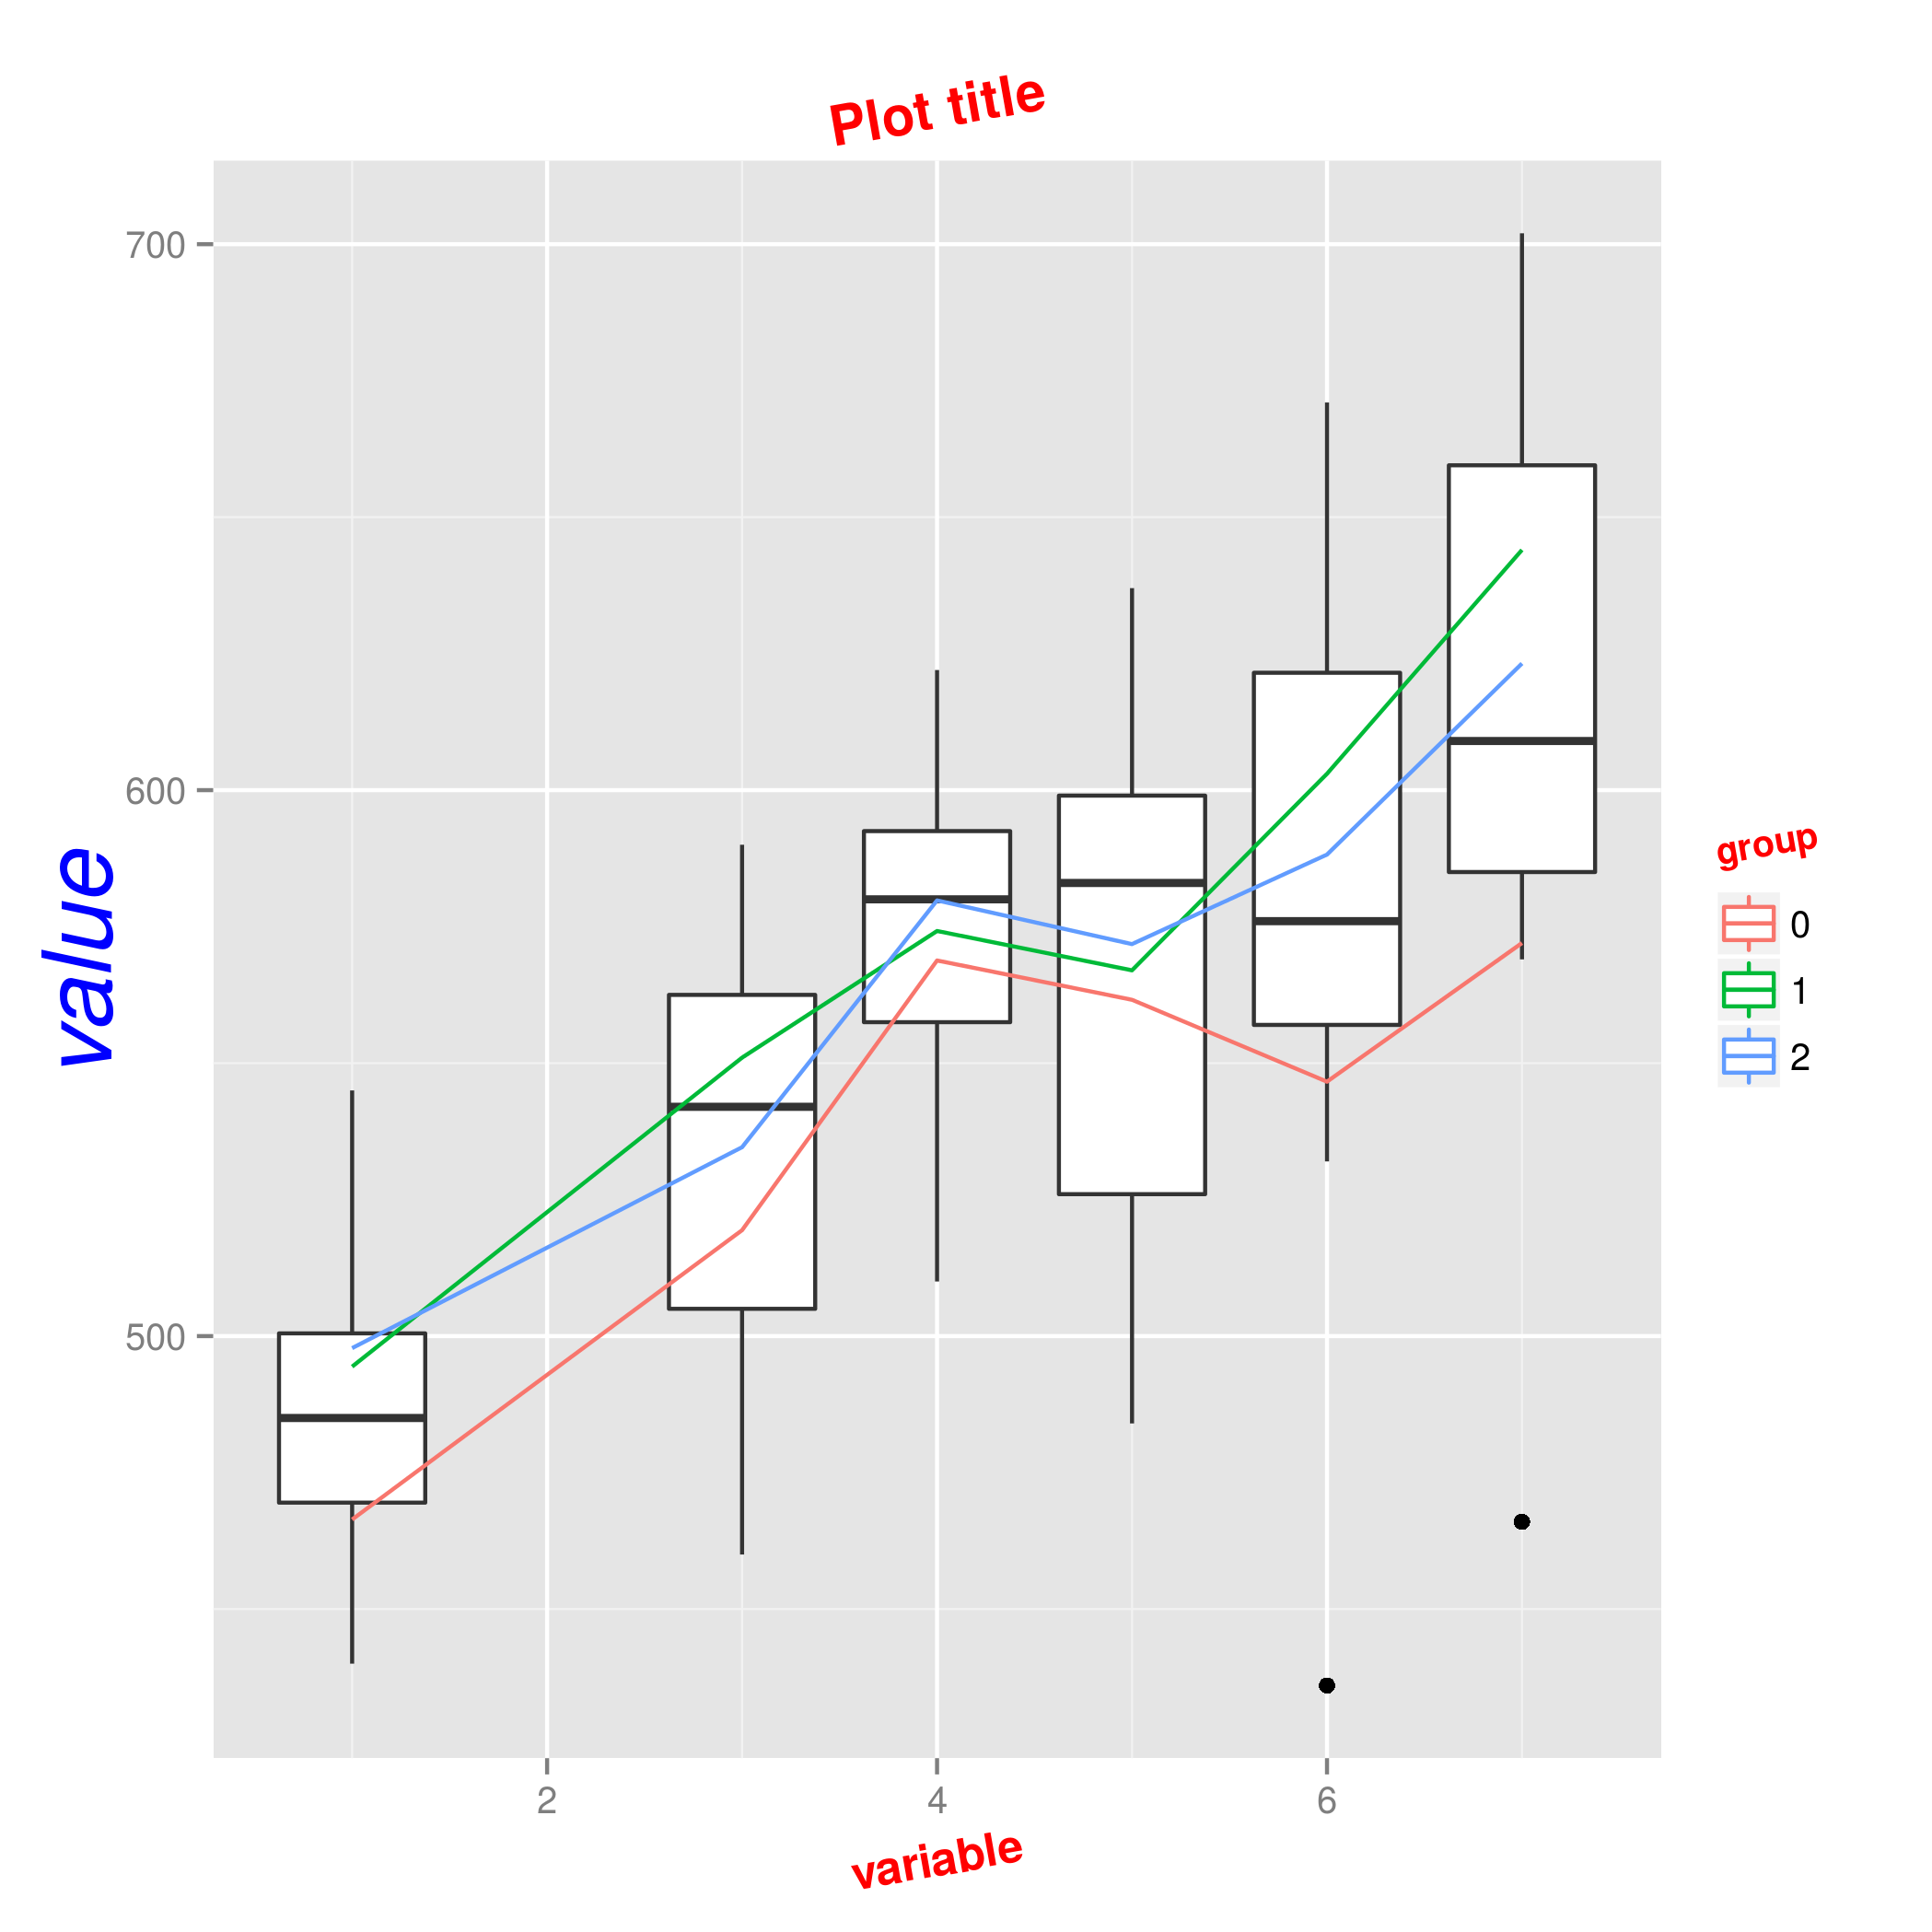
\includegraphics[width=11cm, height=7cm]{ggtext.png}
  \end{center}
\end{frame}



\begin{frame}\frametitle{Line styles}
  \begin{itemize}
  \item the element to modify is an \texttt{element\_line(elem)}
  \item typical elements are:
    \begin{itemize}
    \item \texttt{axis.line.x/y} inherits from \texttt{axis.line}
    \item \texttt{axis.ticks.x/y} inherits from \texttt{text.text}
    \item \texttt{panel.grid.minor/major.x/y} and \texttt{panel.grid}
    \end{itemize}
  \end{itemize}
\end{frame}

\begin{frame}\frametitle{element\_line() options}
  \begin{itemize}
  \item colour: line colour
  \item size: line size
  \item linetype: line type
  \item lineend: line end
  \item color: an alias for ‘colour’ 
  \end{itemize}
\end{frame}


\begin{frame}[fragile,allowframebreaks]\frametitle{Example Data}
\scriptsize
\begin{verbatim}
> p1 + theme(
+     axis.line = element_line(colour="green", linetype = 3, size = 3)
+ )
\end{verbatim}
  \begin{center}
    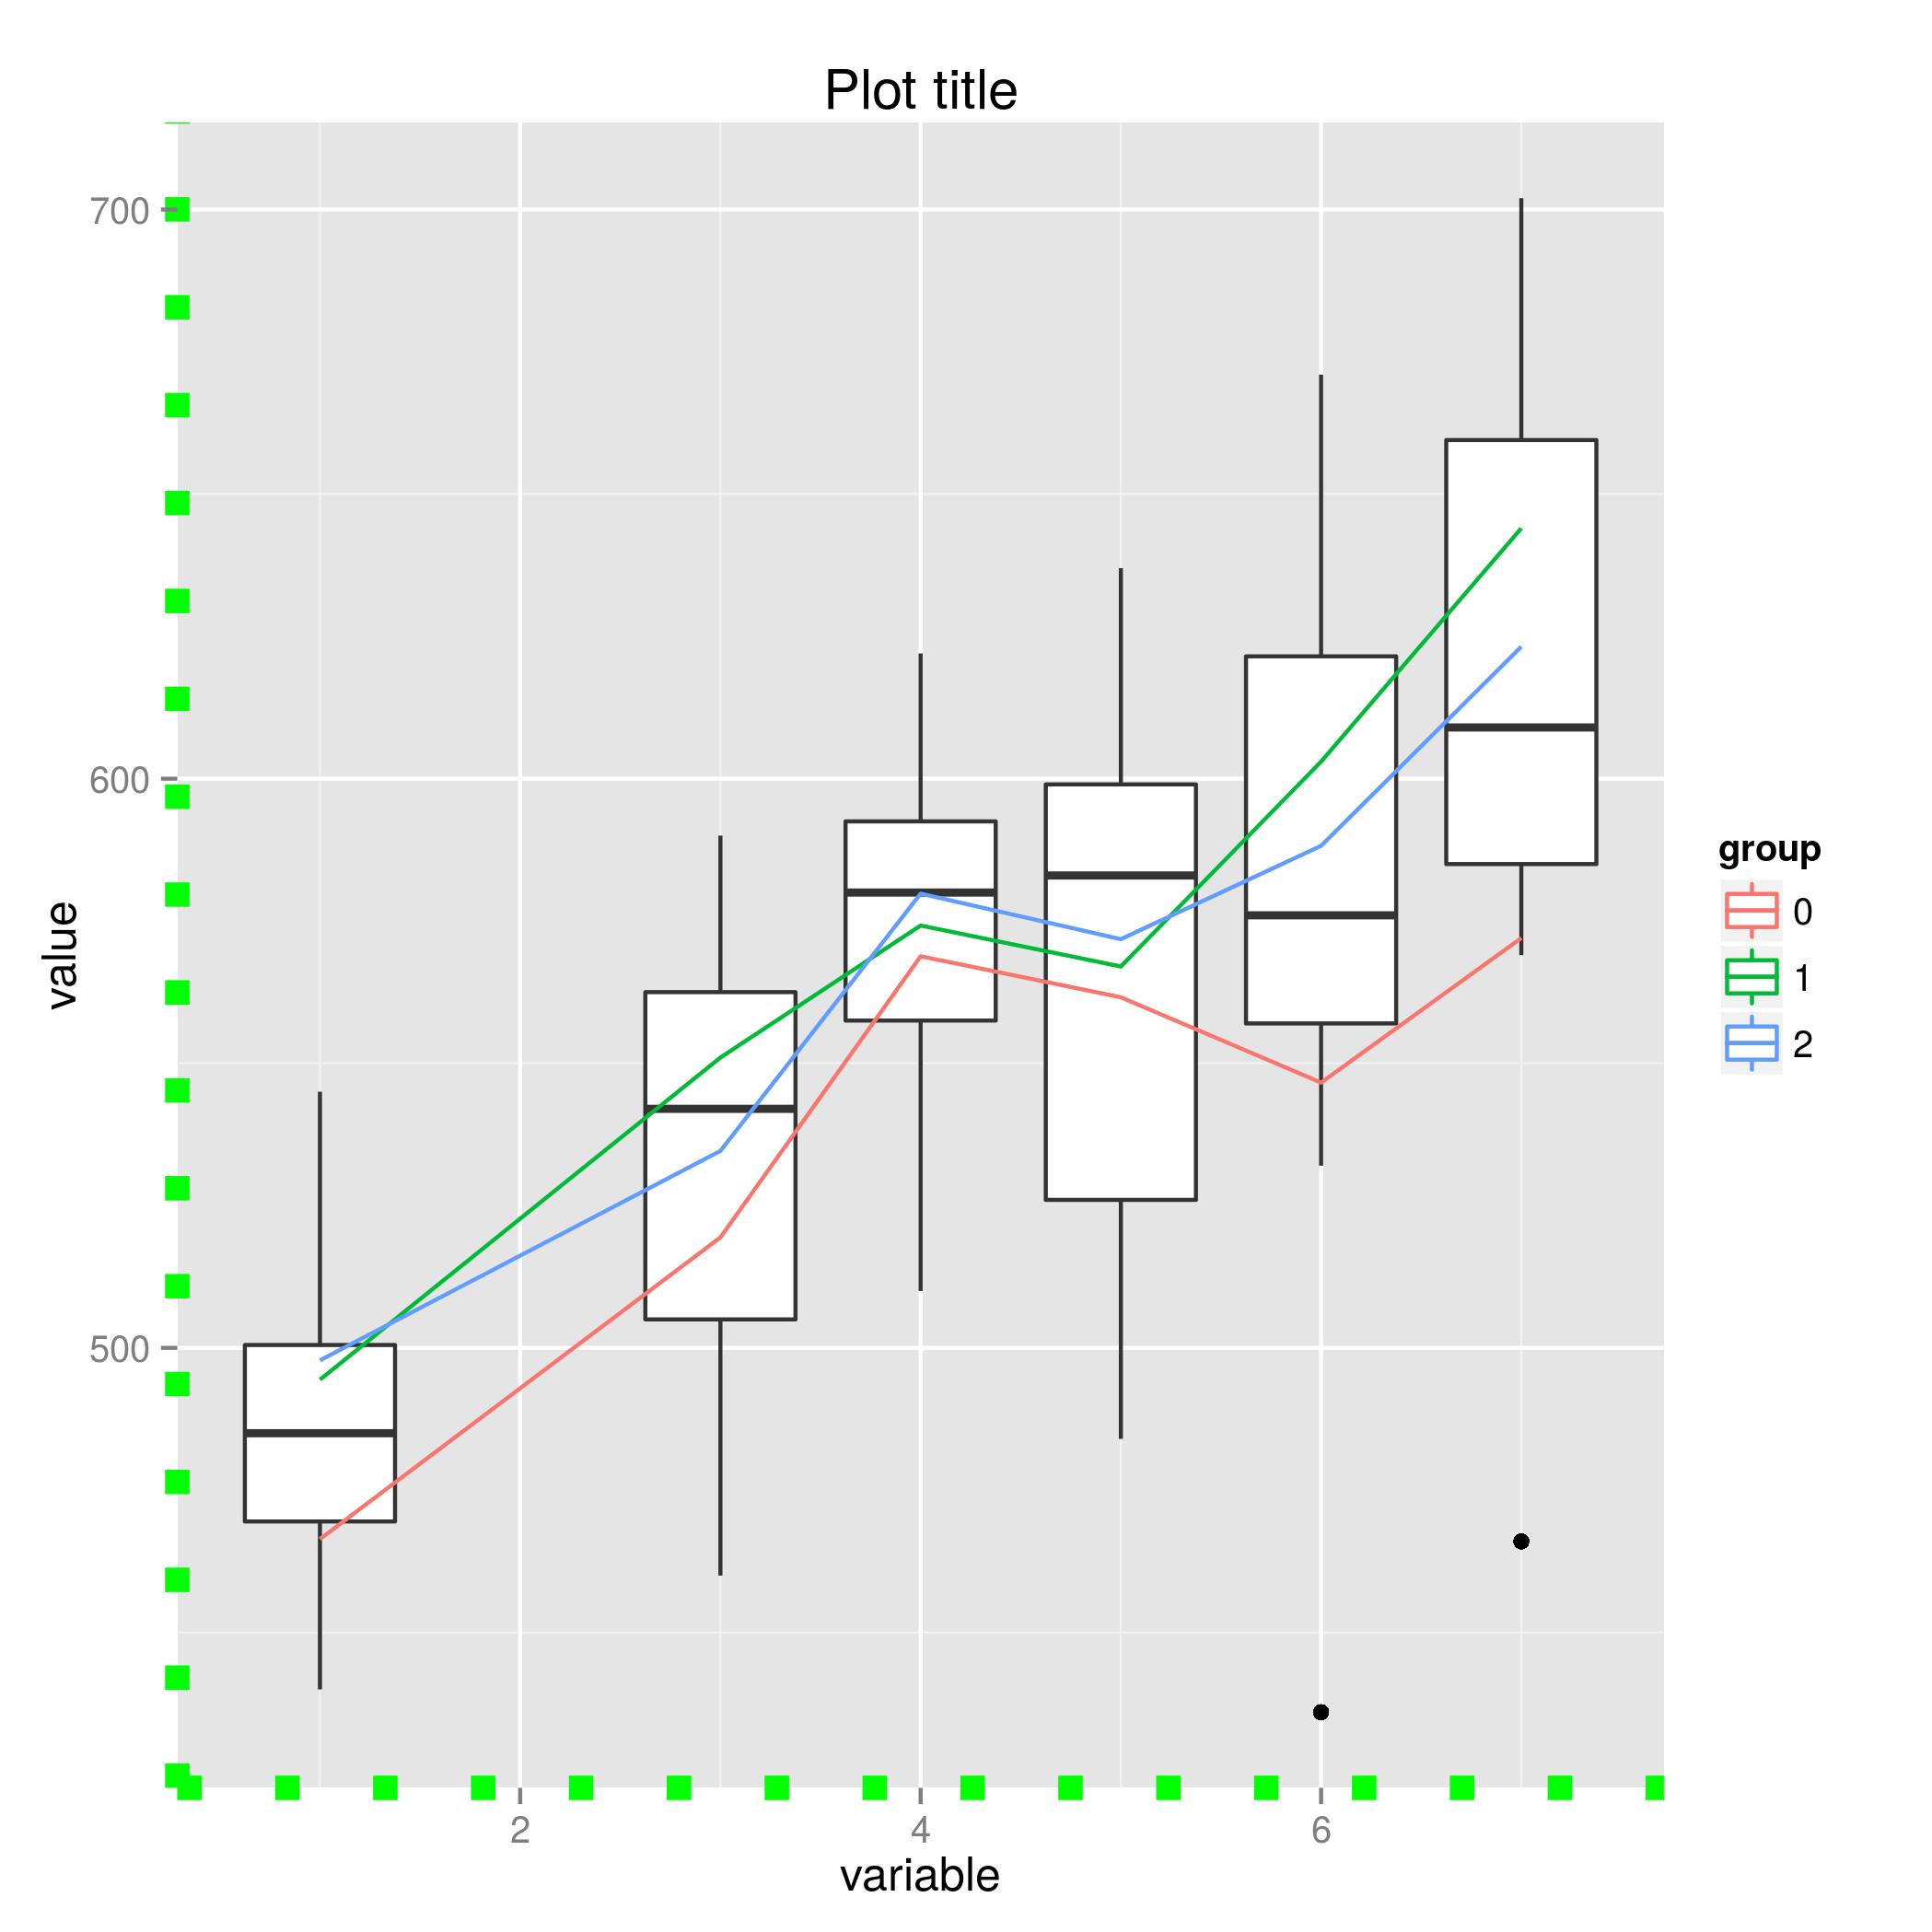
\includegraphics[width=11cm, height=7cm]{ggline.png}
  \end{center}
\end{frame}

\begin{frame}[fragile,allowframebreaks]\frametitle{Example Data}
\scriptsize
\begin{verbatim}
> p1 + theme(
+     axis.line = element_line(colour="green", linetype = 3, size = 3),
+     axis.ticks = element_line(colour="red", linetype = 3, size = 3),
+     panel.grid.major = element_line(colour="deeppink", linetype = 2, size = 1)
+ )
\end{verbatim}
  \begin{center}
    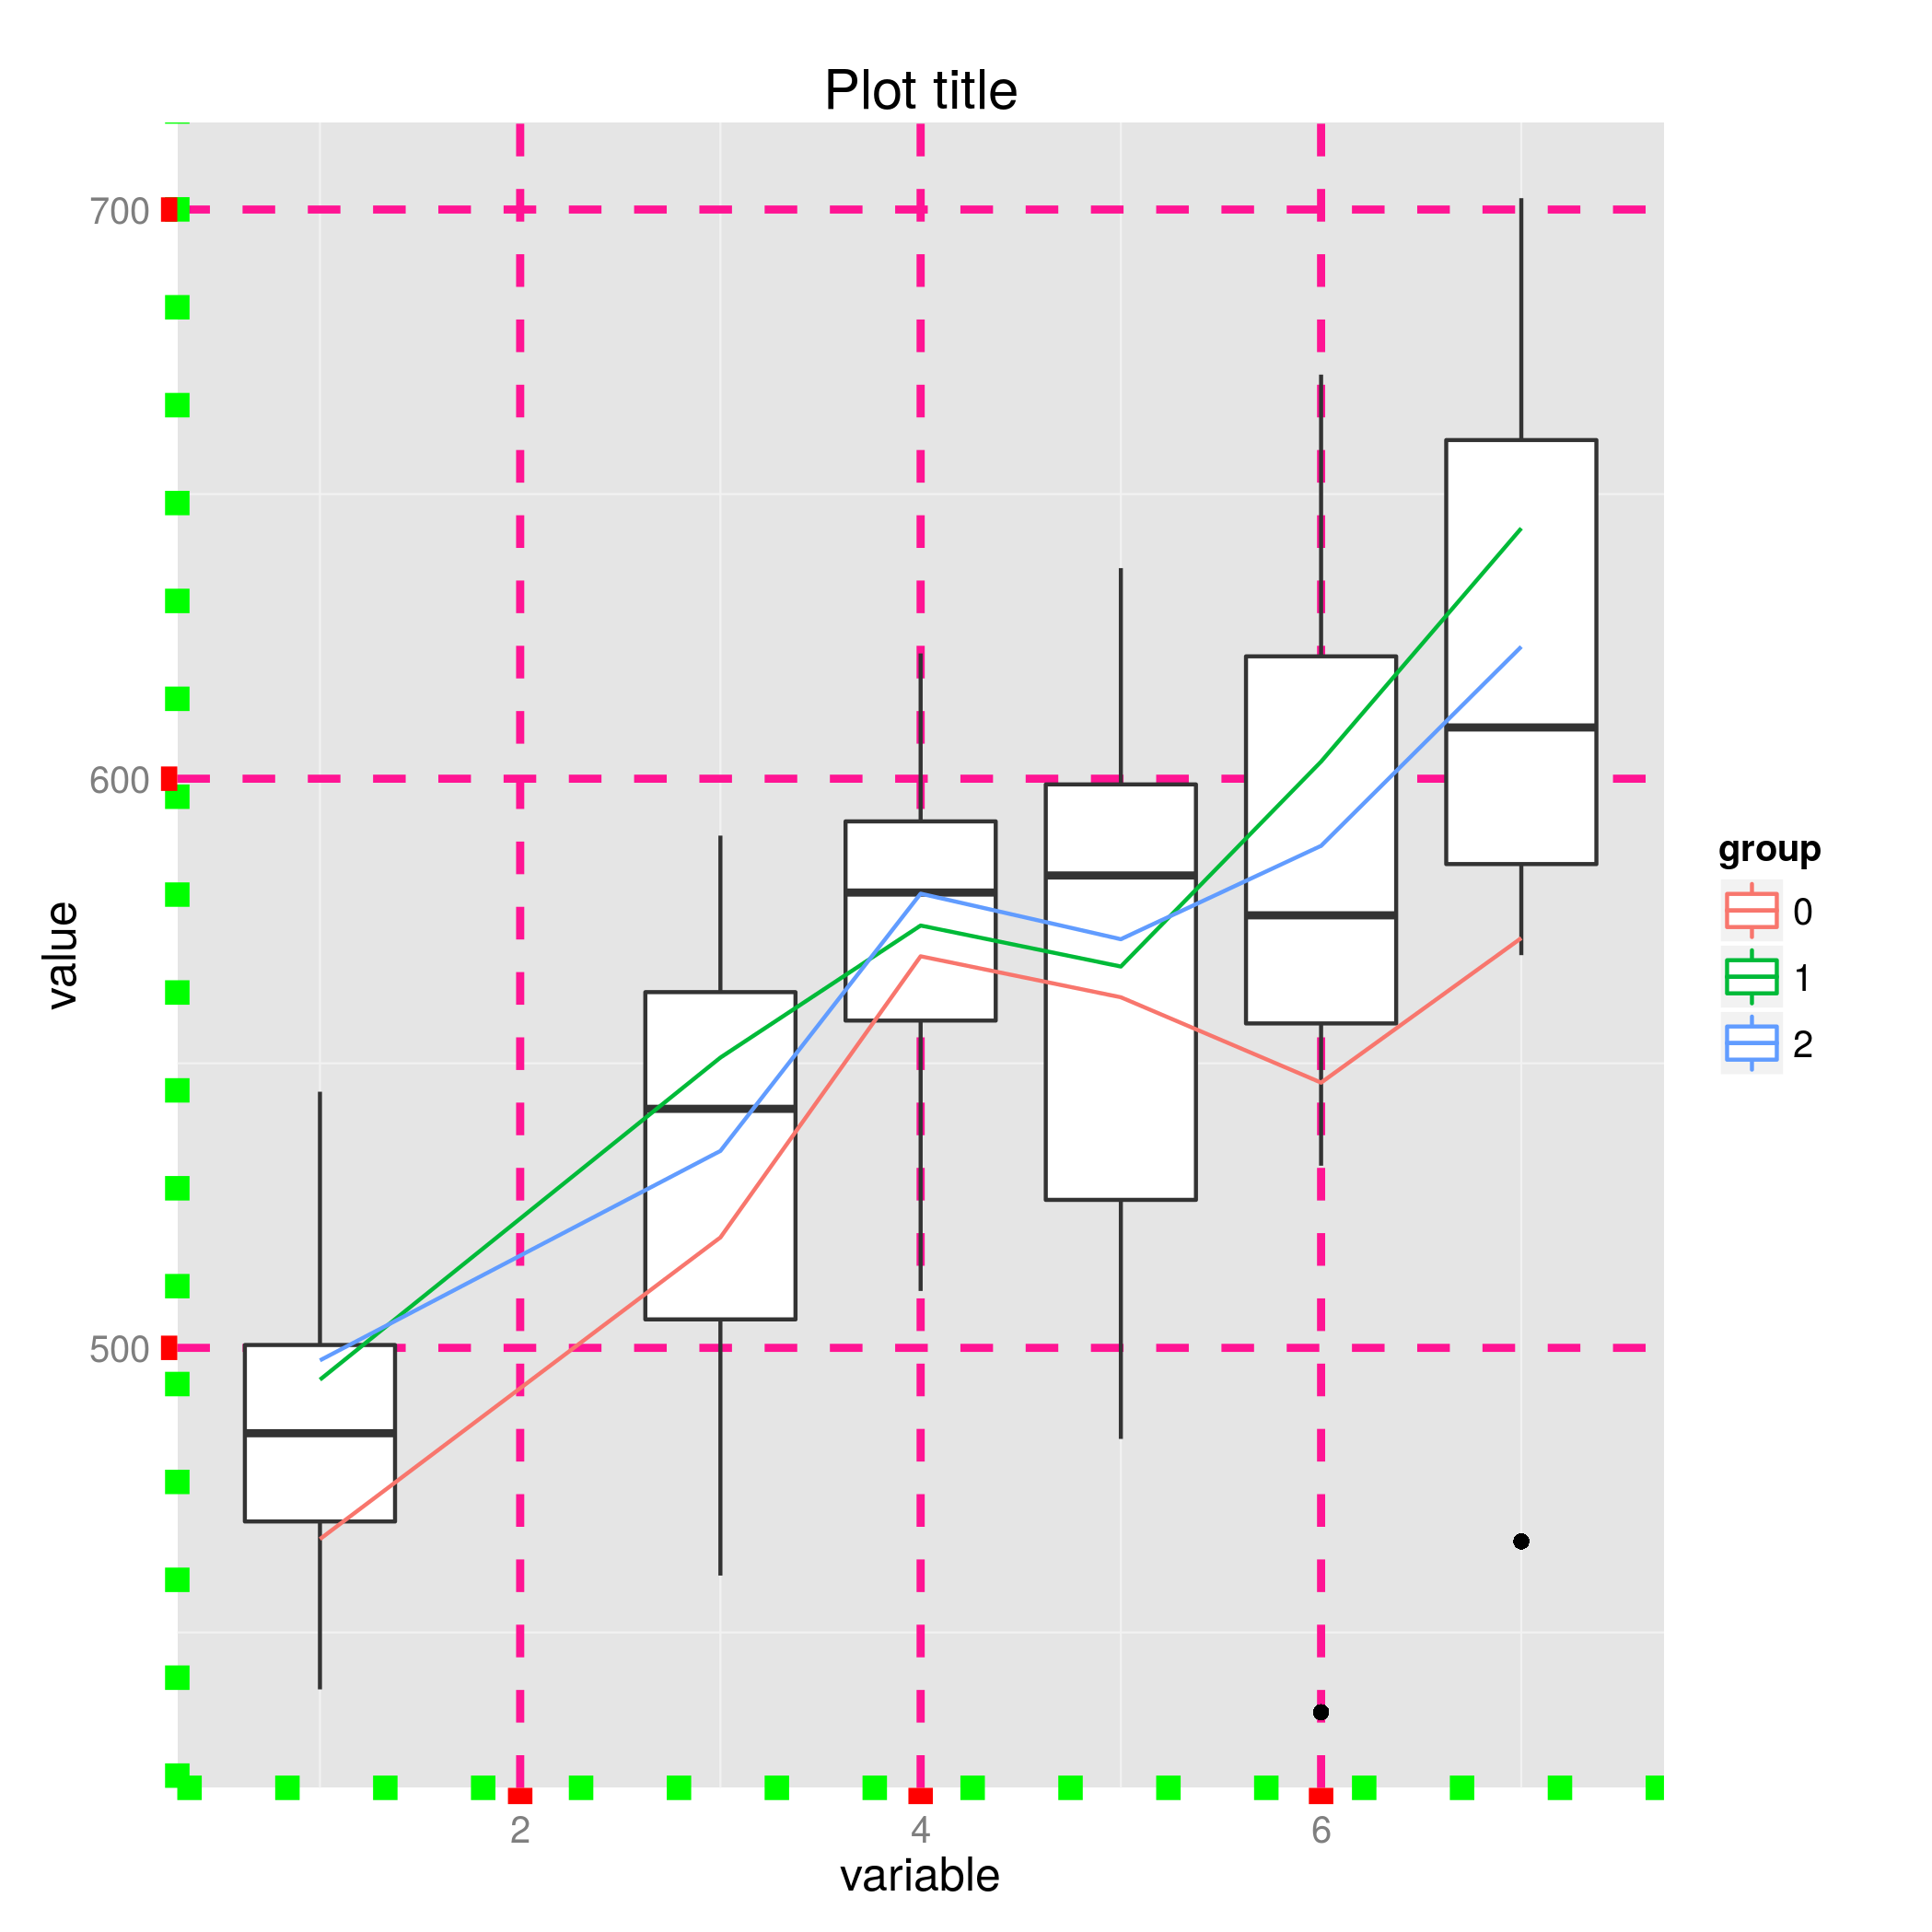
\includegraphics[width=11cm, height=7cm]{ggline2.png}
  \end{center}
\end{frame}



\begin{frame}\frametitle{Rectangular styles}
  \begin{itemize}
  \item the element to modify is an \texttt{element\_rect(elem)}
  \item typical elements are:
    \begin{itemize}
    \item \texttt{legend.background}
    \item \texttt{legend.key} 
    \item \texttt{panel.background}
    \item \texttt{plot.background}
    \item \texttt{strip.background}
    \end{itemize}
  \end{itemize}
\end{frame}

\begin{frame}\frametitle{element\_rect() options}
  \begin{itemize}
  \item fill: fill colour
  \item colour: border colour
  \item size: borer size
  \item linetype: border linetype
  \item color: an alias for ‘colour’ 
  \end{itemize}
\end{frame}


\begin{frame}[fragile,allowframebreaks]\frametitle{Example Data}
\scriptsize
\begin{verbatim}
> p1 + theme(
+     legend.background = element_rect(fill = "darkslategray1"),
+     panel.background = element_rect(fill = "darkslategray3"),
+     plot.background =  element_rect(fill = "darkslateblue")
+ )
\end{verbatim}
  \begin{center}
    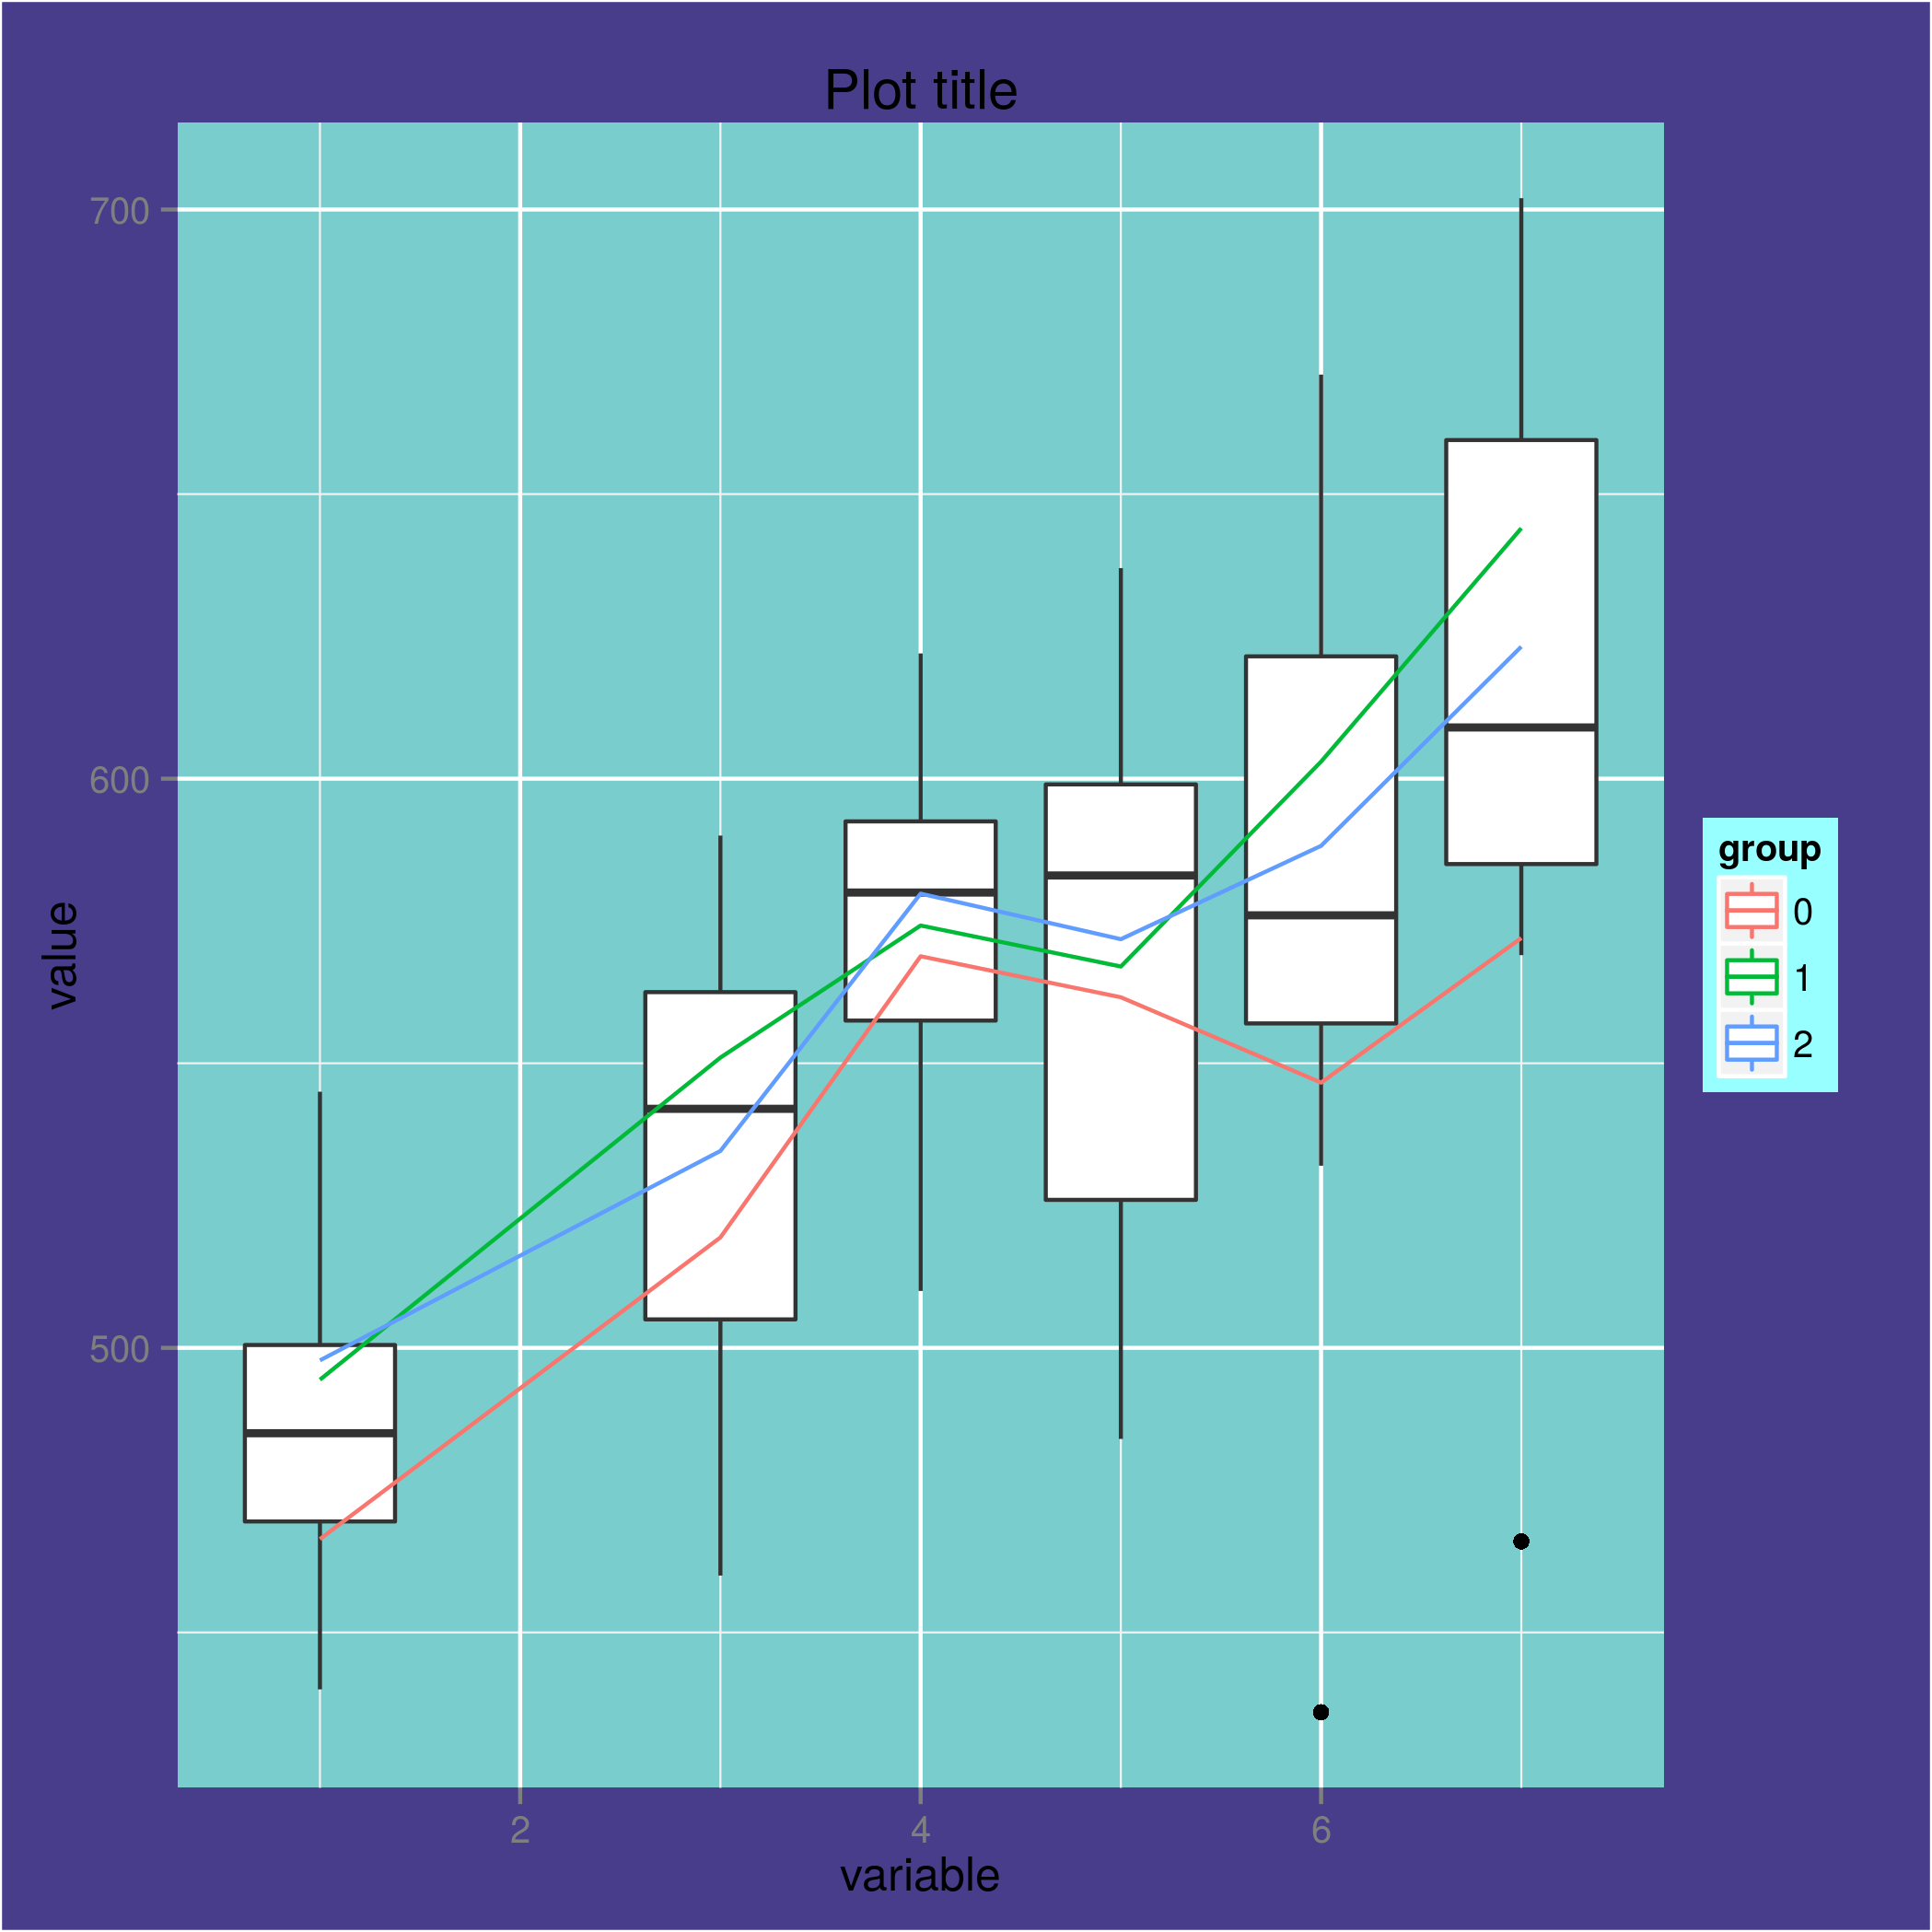
\includegraphics[width=11cm, height=7cm]{ggrect.png}
  \end{center}
\end{frame}



\begin{frame}[allowframebreaks]\frametitle{other options}
  \begin{itemize}
  \item legend.title.align 
  \item legend.position (none,left,right,bottom,top or relative position)
  \item legend.direction (horizontal or vertical)
  \item legend.justification
  \item legend.box (horizontal or vertical - arrangment of multiple legends)
  \item legend.box.just
  \item legend.key.size (unit)
  \item legend.key.height (unit)
  \item legend.key.width (unit)
  \item axis.ticks.length (unit)
  \item axis.ticks.margin (unit)
  \item plot.margin (unit) - margin around the plot
  \item etc
  \end{itemize}
\end{frame}


\begin{frame}[fragile, allowframebreaks]\frametitle{Example Data}
\scriptsize
\begin{verbatim}
> p1 + theme(
+     axis.ticks = element_line(colour="red", linetype = 2, size = 1),
+     axis.ticks.length = unit(1,"cm"),
+     axis.ticks.margin = unit(1,"cm"),
+     legend.position = c(0.5,0.5),
+     legend.background = element_rect(fill="transparent"),
+     legend.key.size = unit(2,"cm")
+ )
\end{verbatim}
  \begin{center}
    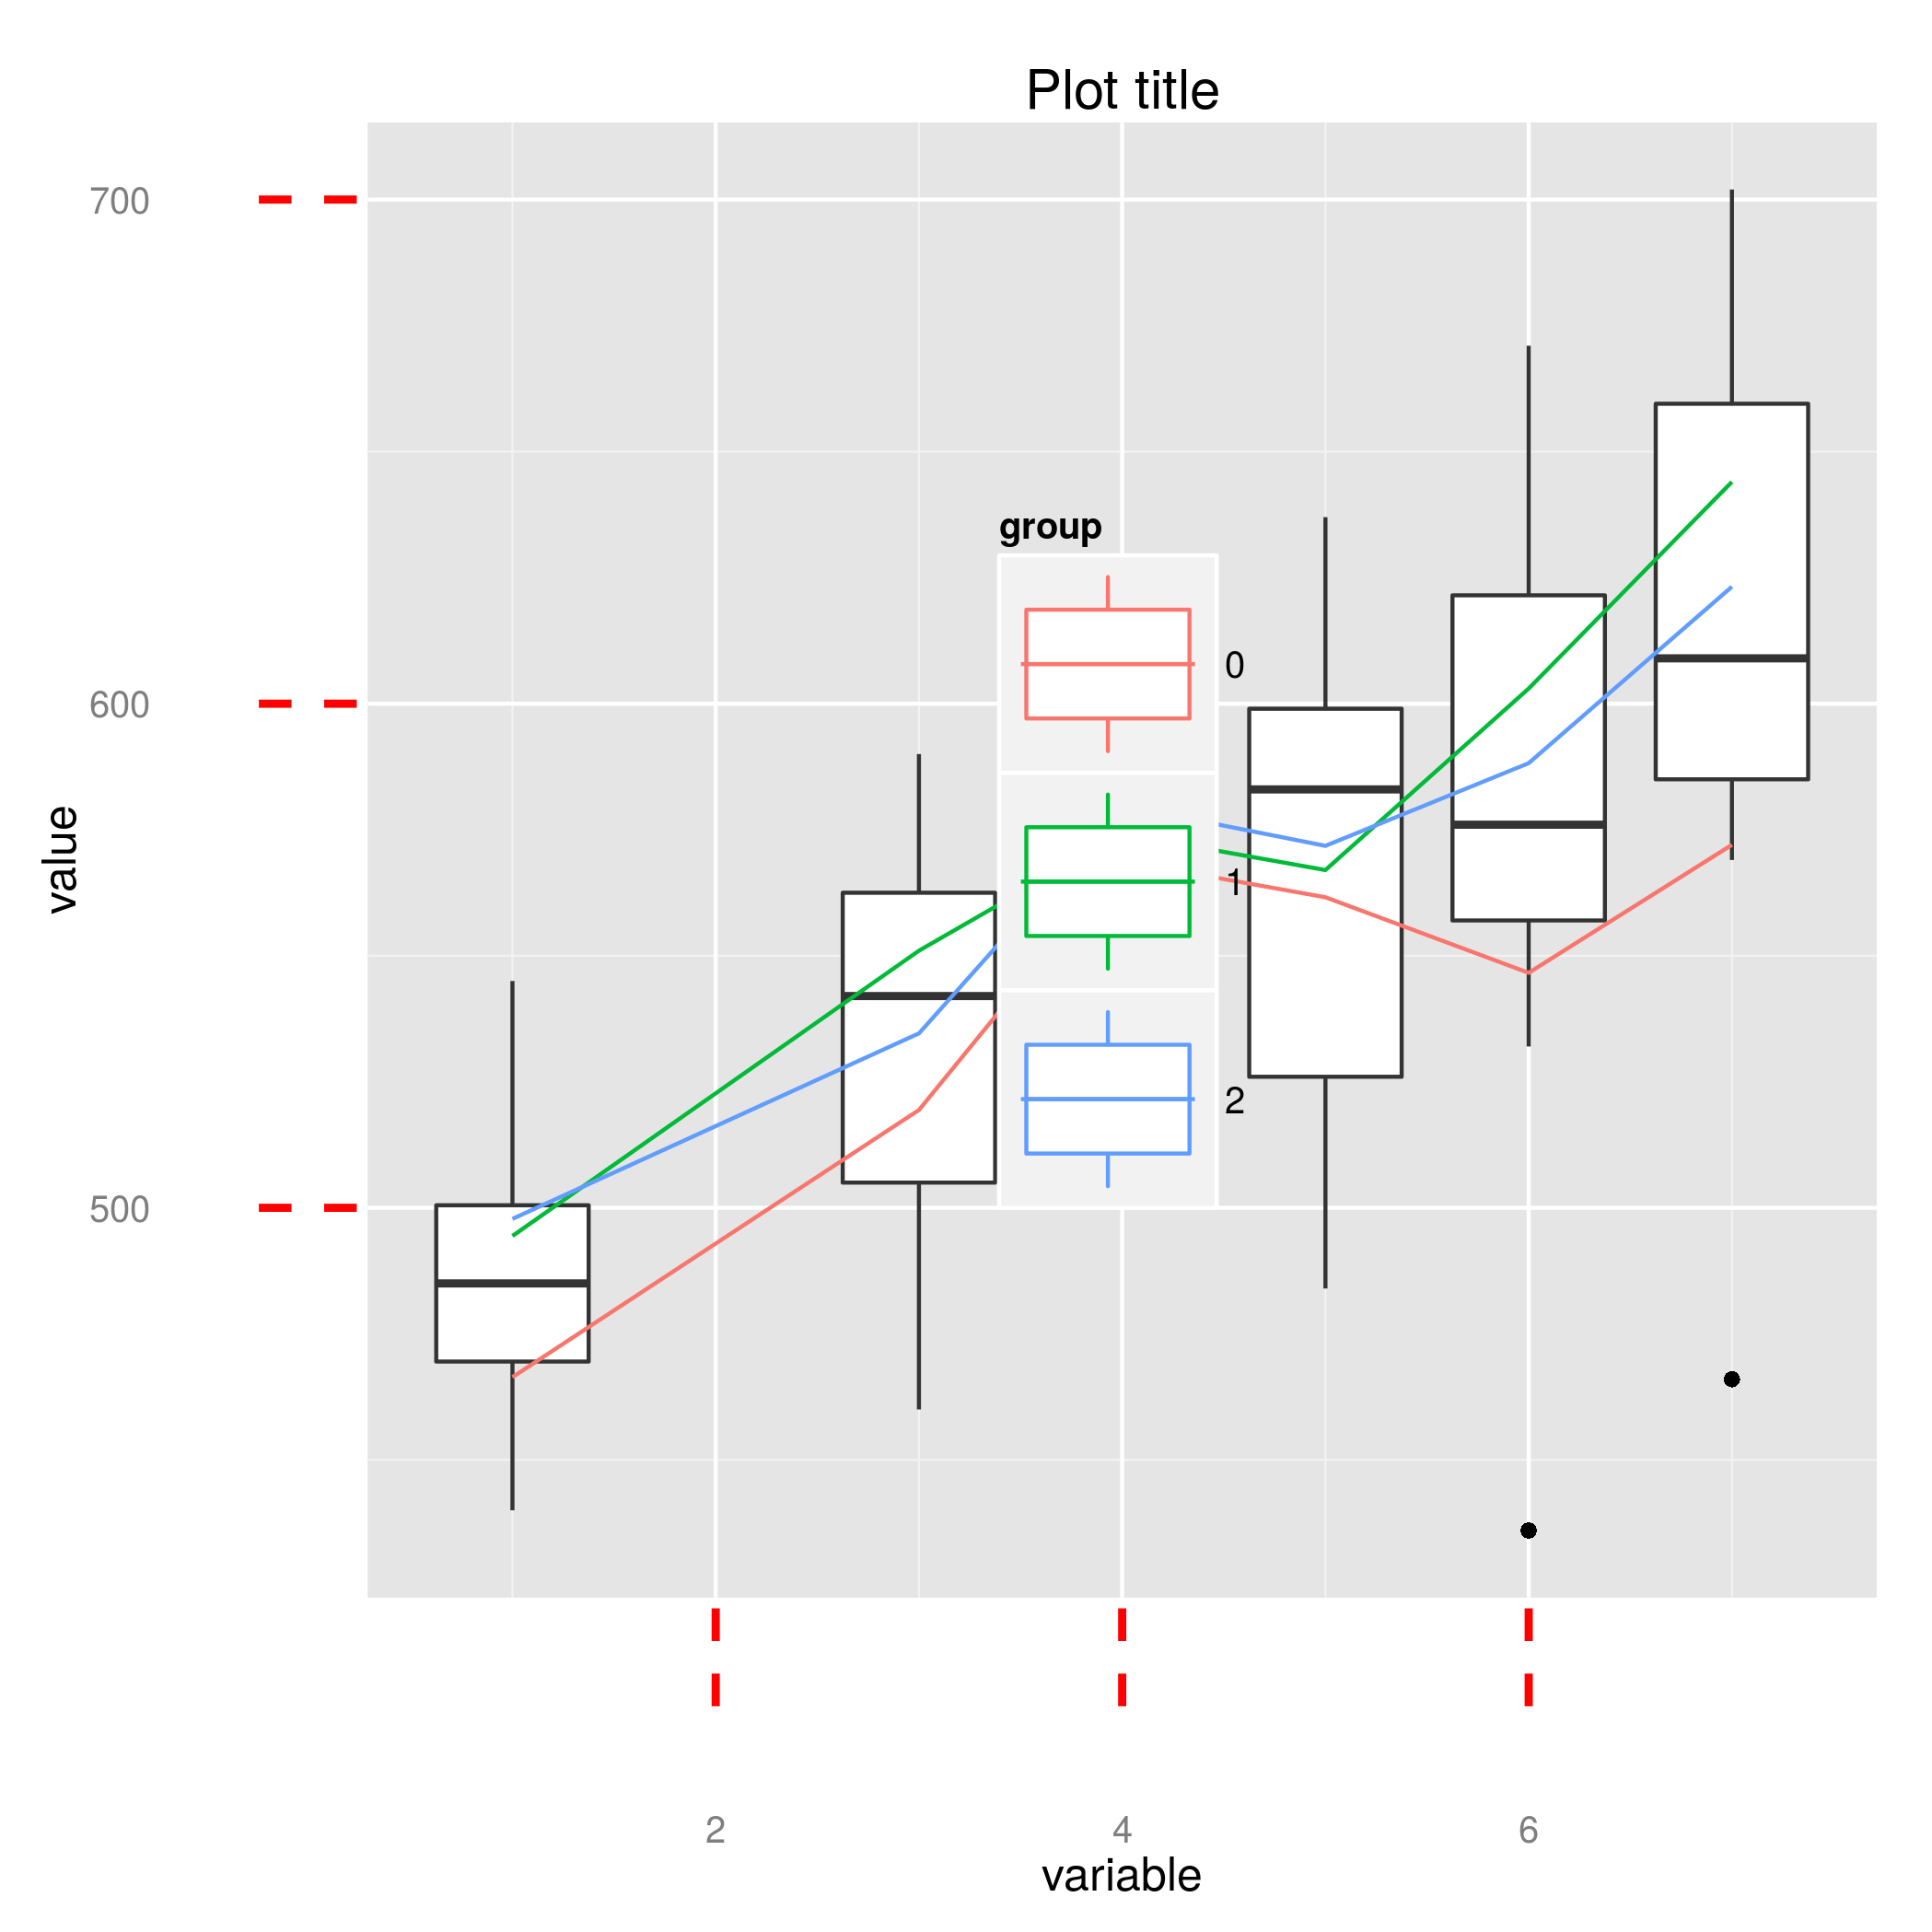
\includegraphics[width=11cm, height=7cm]{ggother.png}
  \end{center}
\end{frame}

\begin{frame}[fragile]\frametitle{Exercises}
  \begin{enumerate}
  \item download the data from the nih:\tiny
\begin{verbatim}
brfss <- read.csv("http://watson.nci.nih.gov/~sdavis/tutorials/IntroToR/BRFSS-subset.csv")  
\end{verbatim}
\normalsize
  \item use dplyr to create a new data frame summarising Age, Height, Weight per Year and Sex, calculate means, min, max, medians, number of observations, number of missing ages
  \item calculate BMI in the brfss data set make an appropriate plot to compare Weight, Height and Age of the sample per Year and sex. Hint: maybe you want transform the data before plotting using melt() from the reshape2 packageadd time as fixed effect.
  \item customize the plot, try to remove all elemets except the boxplot and the text elements
  \item change the colour scale (if you used one)
  \end{enumerate}
\end{frame}


\begin{frame}[fragile,allowframebreaks]\frametitle{Exercises - Solutions}
  \begin{enumerate}
  \item download the data from the nih:\scriptsize
\begin{verbatim}
brfss <- read.csv("http://watson.nci.nih.gov/~sdavis/tutorials/IntroToR/BRFSS-subset.csv")  
\end{verbatim}
\normalsize
  \item use dplyr to create a new data frame summarising Age, Height, Weight per Year and Sex, calculate means, min, max, medians, number of observations, number of missing ages\scriptsize
\begin{verbatim}
> require(dplyr)
> brfss %>% group_by(Sex,Year) %>%
+     summarise(mean.age = mean(Age,na.rm = T),
+               median.age = median(Age,na.rm = T),
+               min.age = min(Age,na.rm = T),
+               max.age = max(Age,na.rm = T),
+               mean.height = mean(Height,na.rm = T),
+               median.height = median(Height,na.rm = T),
+               min.height = min(Height,na.rm = T),
+               max.height = max(Height,na.rm = T),
+               mean.weight = mean(Weight,na.rm = T),
+               median.weight = median(Weight,na.rm = T),
+               min.weight = min(Weight,na.rm = T),
+               max.weight = max(Weight,na.rm = T),
+               nobs = n(),
+               n.missing = sum(is.na(Age)))
Source: local data frame [4 x 16]
Groups: Sex

     Sex Year mean.age median.age min.age max.age mean.height median.height
1 Female 1990 46.23327         42      18      99    163.3367        162.56
2 Female 2010 57.08824         58      18      99    163.2524        163.00
3   Male 1990 43.90552         41      18      94    178.2010        177.80
4   Male 2010 56.24993         57      18      99    178.0066        178.00
Variables not shown: min.height (dbl), max.height (dbl), mean.weight (dbl),
  median.weight (dbl), min.weight (dbl), max.weight (dbl), nobs (int),
  n.missing (int)
\end{verbatim}
\normalsize
  \item calculate BMI in the brfss data set make an appropriate plot to compare Weight, Height and Age of the sample per Year and sex. Hint: maybe you want transform the data before plotting using melt() from the reshape2 packageadd time as fixed effect.
\scriptsize
\begin{verbatim}
> brfss$bmi <- brfss$Weight/(brfss$Height**2) * 10000
> 
> dl <- melt(brfss,id.vars = c("Sex","Year"))
> ggplot(dl,aes(x=factor(Year),y=value,fill=Sex)) +
+     geom_boxplot() +
+     facet_wrap(~variable,scales = "free")
Warnmeldungen:
1: Removed 139 rows containing non-finite values (stat_boxplot). 
2: Removed 649 rows containing non-finite values (stat_boxplot). 
3: Removed 184 rows containing non-finite values (stat_boxplot). 
4: Removed 735 rows containing non-finite values (stat_boxplot).   
\end{verbatim}
  \item customize the plot, try to remove all elemets except the boxplot and the text elements\scriptsize
\begin{verbatim}
> ggplot(dl,aes(x=factor(Year),y=value,fill=Sex)) +
+     geom_boxplot() +
+     facet_wrap(~variable) +
+     theme(
+         plot.background = element_blank(),
+         panel.background = element_blank(),
+         axis.line = element_blank(),
+         axis.ticks = element_blank(),
+         strip.background = element_blank(),
+         panel.grid = element_blank()
+         )
Warnmeldungen:
1: Removed 139 rows containing non-finite values (stat_boxplot). 
2: Removed 649 rows containing non-finite values (stat_boxplot). 
3: Removed 184 rows containing non-finite values (stat_boxplot). 
4: Removed 735 rows containing non-finite values (stat_boxplot).   
\end{verbatim}
\normalsize
  \item change the colour scale (if you used one)\scriptsize
\begin{verbatim}
> ggplot(dl,aes(x=factor(Year),y=value,fill=Sex)) +
+     geom_boxplot() +
+     facet_wrap(~variable) +
+     scale_fill_brewer() +
+     theme(
+         plot.background = element_blank(),
+         panel.background = element_blank(),
+         axis.line = element_blank(),
+         axis.ticks = element_blank(),
+         strip.background = element_blank(),
+         panel.grid = element_blank()
+         )
Warnmeldungen:
1: Removed 139 rows containing non-finite values (stat_boxplot). 
2: Removed 649 rows containing non-finite values (stat_boxplot). 
3: Removed 184 rows containing non-finite values (stat_boxplot). 
4: Removed 735 rows containing non-finite values (stat_boxplot).   
\end{verbatim}
  \end{enumerate}
\end{frame}



\end{document}
